% Options for packages loaded elsewhere
% Options for packages loaded elsewhere
\PassOptionsToPackage{unicode}{hyperref}
\PassOptionsToPackage{hyphens}{url}
\PassOptionsToPackage{dvipsnames,svgnames,x11names}{xcolor}
%
\documentclass[
  letterpaper,
  DIV=11,
  numbers=noendperiod]{scrreprt}
\usepackage{xcolor}
\usepackage{amsmath,amssymb}
\setcounter{secnumdepth}{5}
\usepackage{iftex}
\ifPDFTeX
  \usepackage[T1]{fontenc}
  \usepackage[utf8]{inputenc}
  \usepackage{textcomp} % provide euro and other symbols
\else % if luatex or xetex
  \usepackage{unicode-math} % this also loads fontspec
  \defaultfontfeatures{Scale=MatchLowercase}
  \defaultfontfeatures[\rmfamily]{Ligatures=TeX,Scale=1}
\fi
\usepackage{lmodern}
\ifPDFTeX\else
  % xetex/luatex font selection
\fi
% Use upquote if available, for straight quotes in verbatim environments
\IfFileExists{upquote.sty}{\usepackage{upquote}}{}
\IfFileExists{microtype.sty}{% use microtype if available
  \usepackage[]{microtype}
  \UseMicrotypeSet[protrusion]{basicmath} % disable protrusion for tt fonts
}{}
\makeatletter
\@ifundefined{KOMAClassName}{% if non-KOMA class
  \IfFileExists{parskip.sty}{%
    \usepackage{parskip}
  }{% else
    \setlength{\parindent}{0pt}
    \setlength{\parskip}{6pt plus 2pt minus 1pt}}
}{% if KOMA class
  \KOMAoptions{parskip=half}}
\makeatother
% Make \paragraph and \subparagraph free-standing
\makeatletter
\ifx\paragraph\undefined\else
  \let\oldparagraph\paragraph
  \renewcommand{\paragraph}{
    \@ifstar
      \xxxParagraphStar
      \xxxParagraphNoStar
  }
  \newcommand{\xxxParagraphStar}[1]{\oldparagraph*{#1}\mbox{}}
  \newcommand{\xxxParagraphNoStar}[1]{\oldparagraph{#1}\mbox{}}
\fi
\ifx\subparagraph\undefined\else
  \let\oldsubparagraph\subparagraph
  \renewcommand{\subparagraph}{
    \@ifstar
      \xxxSubParagraphStar
      \xxxSubParagraphNoStar
  }
  \newcommand{\xxxSubParagraphStar}[1]{\oldsubparagraph*{#1}\mbox{}}
  \newcommand{\xxxSubParagraphNoStar}[1]{\oldsubparagraph{#1}\mbox{}}
\fi
\makeatother


\usepackage{longtable,booktabs,array}
\usepackage{calc} % for calculating minipage widths
% Correct order of tables after \paragraph or \subparagraph
\usepackage{etoolbox}
\makeatletter
\patchcmd\longtable{\par}{\if@noskipsec\mbox{}\fi\par}{}{}
\makeatother
% Allow footnotes in longtable head/foot
\IfFileExists{footnotehyper.sty}{\usepackage{footnotehyper}}{\usepackage{footnote}}
\makesavenoteenv{longtable}
\usepackage{graphicx}
\makeatletter
\newsavebox\pandoc@box
\newcommand*\pandocbounded[1]{% scales image to fit in text height/width
  \sbox\pandoc@box{#1}%
  \Gscale@div\@tempa{\textheight}{\dimexpr\ht\pandoc@box+\dp\pandoc@box\relax}%
  \Gscale@div\@tempb{\linewidth}{\wd\pandoc@box}%
  \ifdim\@tempb\p@<\@tempa\p@\let\@tempa\@tempb\fi% select the smaller of both
  \ifdim\@tempa\p@<\p@\scalebox{\@tempa}{\usebox\pandoc@box}%
  \else\usebox{\pandoc@box}%
  \fi%
}
% Set default figure placement to htbp
\def\fps@figure{htbp}
\makeatother


% definitions for citeproc citations
\NewDocumentCommand\citeproctext{}{}
\NewDocumentCommand\citeproc{mm}{%
  \begingroup\def\citeproctext{#2}\cite{#1}\endgroup}
\makeatletter
 % allow citations to break across lines
 \let\@cite@ofmt\@firstofone
 % avoid brackets around text for \cite:
 \def\@biblabel#1{}
 \def\@cite#1#2{{#1\if@tempswa , #2\fi}}
\makeatother
\newlength{\cslhangindent}
\setlength{\cslhangindent}{1.5em}
\newlength{\csllabelwidth}
\setlength{\csllabelwidth}{3em}
\newenvironment{CSLReferences}[2] % #1 hanging-indent, #2 entry-spacing
 {\begin{list}{}{%
  \setlength{\itemindent}{0pt}
  \setlength{\leftmargin}{0pt}
  \setlength{\parsep}{0pt}
  % turn on hanging indent if param 1 is 1
  \ifodd #1
   \setlength{\leftmargin}{\cslhangindent}
   \setlength{\itemindent}{-1\cslhangindent}
  \fi
  % set entry spacing
  \setlength{\itemsep}{#2\baselineskip}}}
 {\end{list}}
\usepackage{calc}
\newcommand{\CSLBlock}[1]{\hfill\break\parbox[t]{\linewidth}{\strut\ignorespaces#1\strut}}
\newcommand{\CSLLeftMargin}[1]{\parbox[t]{\csllabelwidth}{\strut#1\strut}}
\newcommand{\CSLRightInline}[1]{\parbox[t]{\linewidth - \csllabelwidth}{\strut#1\strut}}
\newcommand{\CSLIndent}[1]{\hspace{\cslhangindent}#1}



\setlength{\emergencystretch}{3em} % prevent overfull lines

\providecommand{\tightlist}{%
  \setlength{\itemsep}{0pt}\setlength{\parskip}{0pt}}



 


\KOMAoption{captions}{tableheading}
\makeatletter
\@ifpackageloaded{bookmark}{}{\usepackage{bookmark}}
\makeatother
\makeatletter
\@ifpackageloaded{caption}{}{\usepackage{caption}}
\AtBeginDocument{%
\ifdefined\contentsname
  \renewcommand*\contentsname{Table of contents}
\else
  \newcommand\contentsname{Table of contents}
\fi
\ifdefined\listfigurename
  \renewcommand*\listfigurename{List of Figures}
\else
  \newcommand\listfigurename{List of Figures}
\fi
\ifdefined\listtablename
  \renewcommand*\listtablename{List of Tables}
\else
  \newcommand\listtablename{List of Tables}
\fi
\ifdefined\figurename
  \renewcommand*\figurename{Figure}
\else
  \newcommand\figurename{Figure}
\fi
\ifdefined\tablename
  \renewcommand*\tablename{Table}
\else
  \newcommand\tablename{Table}
\fi
}
\@ifpackageloaded{float}{}{\usepackage{float}}
\floatstyle{ruled}
\@ifundefined{c@chapter}{\newfloat{codelisting}{h}{lop}}{\newfloat{codelisting}{h}{lop}[chapter]}
\floatname{codelisting}{Listing}
\newcommand*\listoflistings{\listof{codelisting}{List of Listings}}
\makeatother
\makeatletter
\makeatother
\makeatletter
\@ifpackageloaded{caption}{}{\usepackage{caption}}
\@ifpackageloaded{subcaption}{}{\usepackage{subcaption}}
\makeatother
\usepackage{bookmark}
\IfFileExists{xurl.sty}{\usepackage{xurl}}{} % add URL line breaks if available
\urlstyle{same}
\hypersetup{
  pdftitle={Orbital Mechanics: Keplerian model},
  pdfauthor={Srihari S},
  colorlinks=true,
  linkcolor={blue},
  filecolor={Maroon},
  citecolor={Blue},
  urlcolor={Blue},
  pdfcreator={LaTeX via pandoc}}


\title{Orbital Mechanics: Keplerian model}
\author{Srihari S}
\date{2025-07-24}
\begin{document}
\maketitle

\renewcommand*\contentsname{Table of contents}
{
\hypersetup{linkcolor=}
\setcounter{tocdepth}{2}
\tableofcontents
}

\bookmarksetup{startatroot}

\chapter*{Preface}\label{preface}
\addcontentsline{toc}{chapter}{Preface}

\markboth{Preface}{Preface}

This book aims to provide a comprehensive guide to the Keplerian model
of orbital mechanics, covering the fundamental principles and equations
governing the motion of celestial bodies. We will explore the historical
context of orbital mechanics, starting with the work of Johannes Kepler
and Isaac Newton, and progressing to modern applications in
astrodynamics and space exploration.

\bookmarksetup{startatroot}

\chapter{Newton's law of gravitation}\label{newtons-law-of-gravitation}

Newton formulated that the gravitational force between two point masses
is directly proportional to the product of their masses and inversely
proportional to the square of the distance between them (inverse square
law):

\[
\vec{F} \propto \frac{m_1 m_2}{r^2} 
\]

\section{How did Newton arrive at the inverse square
law?}\label{how-did-newton-arrive-at-the-inverse-square-law}

Newton deduced the inverse square law through a combination of Kepler's
empirical laws, geometrical analysis, and physical intuition:

\begin{itemize}
\item
  Kepler, building on \textbf{Tycho Brahe}'s detailed astronomical data,
  established these laws:

  \begin{itemize}
  \item
    \textbf{1st Law}: Planets move in elliptical orbits with the Sun at
    one focus.
  \item
    \textbf{2nd Law}: The line joining a planet and the Sun sweeps out
    equal areas in equal time.
  \item
    \textbf{3rd Law}: The square of a planet's orbital period is
    proportional to the cube of its semi-major axis: \(T^2\propto r^3\)
  \end{itemize}
\item
  Newton inferred that the force must be a \textbf{central
  force}---pointing toward the Sun---because Kepler's Second Law (the
  area law) states that a planet sweeps out equal areas in equal time.
  This only happens if the torque about the Sun is zero, which in turn
  implies that the force has no component perpendicular to the radius
  vector. Therefore, the force must always point along the line joining
  the planet and the Sun---making it a central force.
\item
  \textbf{Deriving the inverse-square relationship:} Starting with
  Kepler's Third law:
  \(T^2 \propto r^3 \Rightarrow \left(\frac{2\pi r}{v}\right)^2 \propto r^3 \Rightarrow v^2 \propto \frac{1}{r} \Rightarrow a= \frac{v^2}{r} \propto \frac{1}{r^2}\)
  This showed Newton that the acceleration required to keep a planet in
  orbit must follow an inverse-square law
\item
  To test the universality of this law, Newton compared the
  gravitational acceleration near Earth's surface (
  \(a_E\approx 9.81 m/s^2\)) with the centripetal acceleration needed to
  keep the Moon in its orbit using the following measurements to
  calculate the velocity in its orbit:

  \begin{itemize}
  \tightlist
  \item
    The Moon's distance from the Earth: about 60 Earth radii (or 384,400
    km).
  \item
    And the orbital period was around 27.3 days.
  \end{itemize}

  And he found:
  \(\frac{a_E}{a_M}\approx \left(\frac{r_M}{r_E} \right)^2\) . This
  confirmed that the same law governed both falling of objects near
  Earth as well as orbiting moons.
\end{itemize}

\bookmarksetup{startatroot}

\chapter{Two Body Problem}\label{two-body-problem}

\section{Equations of Motion for the Two body
problem}\label{equations-of-motion-for-the-two-body-problem}

Let \(\vec{R}_1\) and \(\vec{R}_2\) denote the position vectors of
masses \(m_1\) and \(m_2\) in an inertial reference frame. According to
Newton's Second Law and the law of gravitation:

\begin{equation}\phantomsection\label{eq-f12}{
m_1\ddot{\vec{R}}_1=-G\frac{m_1 m_2}{r^3} \vec{r}
}\end{equation}

\begin{equation}\phantomsection\label{eq-f21}{
m_2\ddot{\vec{R}}_2=G\frac{m_1 m_2}{r^3} \vec{r}
}\end{equation}

where \(\vec{r}= \vec{R}_2-\vec{R}_1\).

\begin{figure}[H]

{\centering 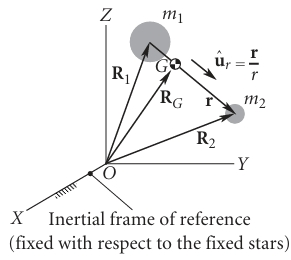
\includegraphics[width=2.63542in,height=\textheight,keepaspectratio]{fig2_1.jpeg}

}

\caption{Diagram of two masses in an inertial frame \emph{OXYZ} (Curtis
(2005))}

\end{figure}%

\subsection{Deriving the relative equation of
motion}\label{deriving-the-relative-equation-of-motion}

Substituting Equation~\ref{eq-f12} and Equation~\ref{eq-f21} to
\(\vec{r}= \vec{R}_2-\vec{R}_1\):

\(\ddot{\vec{r}}= -G\frac{m_1 m_2}{r^3}\vec{r}\left(\frac{1}{m_2}+\frac{1}{m_1}\right)= -G \frac{m_1+m_2}{r^3} \vec{r}\)

Let the gravitational 𝜇 parameter be defined as:

\[
\mu= G(m_1+m_2)
\]

Hence the final equation that we use turns out to be:

\begin{equation}\phantomsection\label{eq-relmotion}{
\boxed{\ddot{\vec{r}}=-\frac{\mu}{r^3}\vec{r}}
}\end{equation}

\subsection{Motion of Center of Mass}\label{motion-of-center-of-mass}

The center of mass vector is:
\(\vec{R}_G=\frac{m_1\vec{R}_1+m_2\vec{R}_2}{m_1+m_2}\)

Using Equation~\ref{eq-f12} and Equation~\ref{eq-f21} :

\begin{equation}\phantomsection\label{eq-com}{
\ddot{\vec{R}}_G= \frac{m_1\ddot{\vec{R}}_1+m_2\ddot{\vec{R}}_2}{m_1+m_2}
}\end{equation}

\[
\ddot{\vec{R}}_G=\frac{-G\frac{m_1m_2}{r^3}\vec{r}+G\frac{m_1m_2}{r^3}\vec{r}}{m_1+m_2}=0
\]

Hence proved that the acceleration of center of mass is zero.

\section{Angular momentum in two body problem}\label{sec-angularmom}

The angular momentum of body \(m_2\) relative to \(m_1\) is moment of
\(m_2\)'s relative linear momentum \(m_2 \dot{\vec{r}}\):

\[
\vec{H}_{2/1}= \vec{r} \times m_2\dot{\vec{r}}
\]

where \(\dot{\vec{r}}\) is the velocity of \(m_2\) relative to \(m_1\).
We divide this equation of the mass term and get the specific relative
angular momentum:

\[
\vec{h}= \vec{r}\times\dot{\vec{r}}
\]

On calculating the time derivative:

\[
\frac{d\vec{h}}{dt}=\dot{\vec{r}}\times\dot{\vec{r}}+ \vec{r}\times \ddot{\vec{r}}
\]

From the Equation~\ref{eq-relmotion}, we see that
\(\ddot{\vec{r}} \parallel \vec{r}\) . Hence
\(\frac{d\vec{h}}{dt}=0 \Rightarrow \vec{h}\) is conserved.

\subsection{Eccentricity of orbit from Laplace Runge Lenz
vector}\label{eccentricity-of-orbit-from-laplace-runge-lenz-vector}

Differentiating \(\dot {\vec r} \times \vec h\):

\begin{equation}\phantomsection\label{eq-init}{
\frac{d}{dt}(\dot{\vec r}\times\vec h)= \ddot{\vec r}\times\vec h + \dot{\vec r}\times\underbrace{\dot{\vec h}}_{0}= -\frac{\mu}{r^{3}}\vec r\times(\vec r\times\dot{\vec r})
}\end{equation}

Using the triple product identity
\(\vec{a}\times(\vec{b}\times\vec{c})=(\vec{a}\cdot\vec{c})\vec b-(\vec a \cdot \vec b)\vec c\)
:

\[
\vec r\times(\vec r\times\dot{\vec r})= (\vec r\cdot\dot{\vec r})\vec r - r^{2}\dot{\vec r}
\]

And using the identity \(\vec r \cdot \dot{\vec r}=r\dot r\)(See
\textbf{?@sec-appendix} ), we get:

\begin{equation}\phantomsection\label{eq-rcrossrcrossrdot}{ 
\vec r\times(\vec r\times\dot{\vec r})= (r\dot r)\vec r - r^{2}\dot{\vec r} 
}\end{equation}

Inserting Equation~\ref{eq-rcrossrcrossrdot} into Equation~\ref{eq-init}
:

\begin{equation}\phantomsection\label{eq-six}{
\frac{d}{dt}(\dot{\vec r}\times \vec h)=- \frac{\mu}{r^3}\left[(r \dot{r})\vec r - r^2 \dot{\vec r}\right]=-\mu \left[\frac{\dot r \vec r-r\dot{\vec r}}{r^2}\right]
}\end{equation}

But ,

\[
\frac{d}{dt}\left(\frac{\vec r}{r}\right)= \frac{r\dot{\vec r}-\dot r\vec r}{r^2}=-\frac{\dot r\vec r-r\dot{\vec r}}{r^2}
\]

substituting the above into Equation~\ref{eq-six};

\[
\frac{d}{dt}\left(\dot{\vec r}\times \vec h\right)= \frac{d}{dt}\left(\mu\frac{\vec r}{r}\right)
\]

Which on integration, gives this solution:

\begin{equation}\phantomsection\label{eq-eccvector}{
\frac{1}{\mu}(\dot{\vec{r}}\times \vec h)-\frac{\vec r}{r}=\vec e
}\end{equation}

where \(\vec e\) is the constant of integration and called as the
Laplace-Runge-Lenz Vector. The significance of this vector is that its
magnitude \(|\vec e|\) gives the eccentricity \(e\) and it faces in the
direction of the periapsis of the orbit.

\section{Orbit Equation (Trajectory Under
Gravity)}\label{orbit-equation-trajectory-under-gravity}

Equation~\ref{eq-eccvector} is the vector equation that represents the
relative motion of one body wrt the other in two body problem. In order
to obtain the scalar form, we take a dot product with \(\vec r\):

\[
\frac{1}{\mu}(\dot{\vec{r}}\times \vec h)\cdot \vec r-\frac{\vec r\cdot \vec r}{r}=\vec e\cdot \vec r
\]

Using the identity
\(\vec a \cdot (\vec b \times \vec c)=(\vec a \times \vec b)\cdot \vec c\);

\[
\frac{1}{\mu}\underbrace{(\vec r \times \dot{\vec r})}_{\vec h}\cdot \vec h- \frac{\vec r\cdot\vec r}{r}=\vec e\cdot\vec r
\]

\[
\frac{h^2}{\mu}-r=re\cos{\theta} \text{ where } \theta \text{ is the true anomaly angle }
\]

\begin{figure}[H]

{\centering 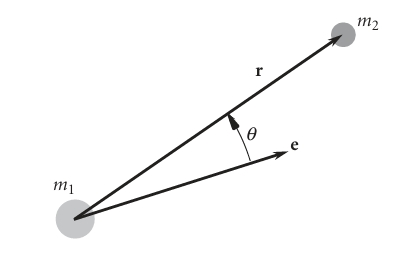
\includegraphics[width=2.40625in,height=\textheight,keepaspectratio]{fig2_2.jpeg}

}

\caption{The true anomaly \(\theta\) is the angle between the
eccentricity vector \(\vec{e}\) and the position vector \(\vec{r}\).}

\end{figure}%

Hence the final equation of orbit will turn out to be as follows:

\[
\boxed{r=\frac{\frac{h^2}{\mu}}{1+e\cos{\theta}}}
\]

\section{Two body problem simulation}\label{two-body-problem-simulation}

\bookmarksetup{startatroot}

\chapter*{Appendix}\label{sec-appendix}
\addcontentsline{toc}{chapter}{Appendix}

\markboth{Appendix}{Appendix}

\section*{Table of equations}\label{table-of-equations}
\addcontentsline{toc}{section}{Table of equations}

\markright{Table of equations}

\begin{longtable}[]{@{}
  >{\raggedright\arraybackslash}p{(\linewidth - 2\tabcolsep) * \real{0.3472}}
  >{\raggedright\arraybackslash}p{(\linewidth - 2\tabcolsep) * \real{0.6528}}@{}}
\toprule\noalign{}
\begin{minipage}[b]{\linewidth}\raggedright
Quantity
\end{minipage} & \begin{minipage}[b]{\linewidth}\raggedright
Equation
\end{minipage} \\
\midrule\noalign{}
\endhead
\bottomrule\noalign{}
\endlastfoot
Ellipse & \(r=\dfrac{p}{1+e\cos\theta}\) \\
Area law &
\(\dot A=\frac12 r^{2}\dot\theta =\frac{h}{2}= \text{const}\) \\
Harmonic law & \(T^{2}\propto a^{3}\) \\
Gravity & \(\vec F_{21} = -\dfrac{Gm_{1}m_{2}}{r^{2}}\hat{u_r}\) \\
Reduced EoM & \(\ddot{\vec r}=-\dfrac{\mu}{r^{3}}\vec r\) \\
Specific angular momentum & \(\vec h=\vec r\times\dot{\vec r}\) \\
Laplace--Runge--Lenz vector &
\(\vec e=\dfrac{\dot{\vec r}\times\vec h}{\mu}-\dfrac{\vec r}{r}\) \\
\end{longtable}

\section*{Identities derivation}\label{identities-derivation}
\addcontentsline{toc}{section}{Identities derivation}

\markright{Identities derivation}

\subsection*{\texorpdfstring{1.
\(\vec{r}\cdot \dot{\vec{r}}=r\dot{r}\)}{1. \textbackslash vec\{r\}\textbackslash cdot \textbackslash dot\{\textbackslash vec\{r\}\}=r\textbackslash dot\{r\}}}\label{vecrcdot-dotvecrrdotr}
\addcontentsline{toc}{subsection}{1.
\(\vec{r}\cdot \dot{\vec{r}}=r\dot{r}\)}

We know that: \(\vec{r}\cdot\vec{r}=r^2\). Then : \[
\frac{d}{dt}(\vec{r} \cdot \vec{r})=2r \frac{dr}{dt}=2r\dot{r}
\]

But,

\[
\frac{d}{dt}(\vec r\cdot \vec r)= \vec r\cdot \frac{d\vec r}{dt}+\frac{d\vec r}{dt}\cdot \vec r= 2\vec r\cdot \frac{d\vec r}{dt}=2\vec r\cdot \dot{\vec r}
\]

Hence: \[\boxed{\vec r \cdot\dot{\vec r}=r\dot r}\]

\bookmarksetup{startatroot}

\chapter*{References}\label{references}
\addcontentsline{toc}{chapter}{References}

\markboth{References}{References}

\phantomsection\label{refs}
\begin{CSLReferences}{1}{0}
\bibitem[\citeproctext]{ref-curtis2005orbital}
Curtis, H. D. 2005. \emph{Orbital Mechanics: For Engineering Students}.
Aerospace Engineering. Elsevier Science.
\url{https://books.google.co.in/books?id=nEO7lAEACAAJ}.

\end{CSLReferences}




\end{document}
